
\subsection{2分ヒープ}
\frame{
  \frametitle{2分ヒープ}
  \begin{block}{Binary Heap}
    全順序集合$P(C,\leq)$について,$C$上の要素からなるヒープは\\
    以下の操作が実行できる
    \itemize{
    \item push : $O(\log N)$で$C$の要素$x$を追加する
    \item replace : $O(\log N)$で$C$の要素$x$でヒープの最大値をもつ要素を置き換える
    \item pop : $O(\log N)$でヒープの最大値をもつ要素を削除する
    \item delete : $O(1)$で与えられたポインタの先の要素を消去する
    \item top : $O(1)$でヒープの最大値を求める\\
    }
    ヒープ条件を満たす完全二分木の構造\\
    (二分木:出次数が高々2の有向木)\\
    (完全二分木:出次数が0か2で,全ての葉が同じ深さ)
  \end{block}
}

\frame{
  \frametitle{2分ヒープ}
  \begin{alertblock}{ヒープ条件}
    \center{
      全ての要素の値はその親の要素の値より小さいか等しい
    }
  \end{alertblock}
  \begin{exampleblock}{例}
    \center{
      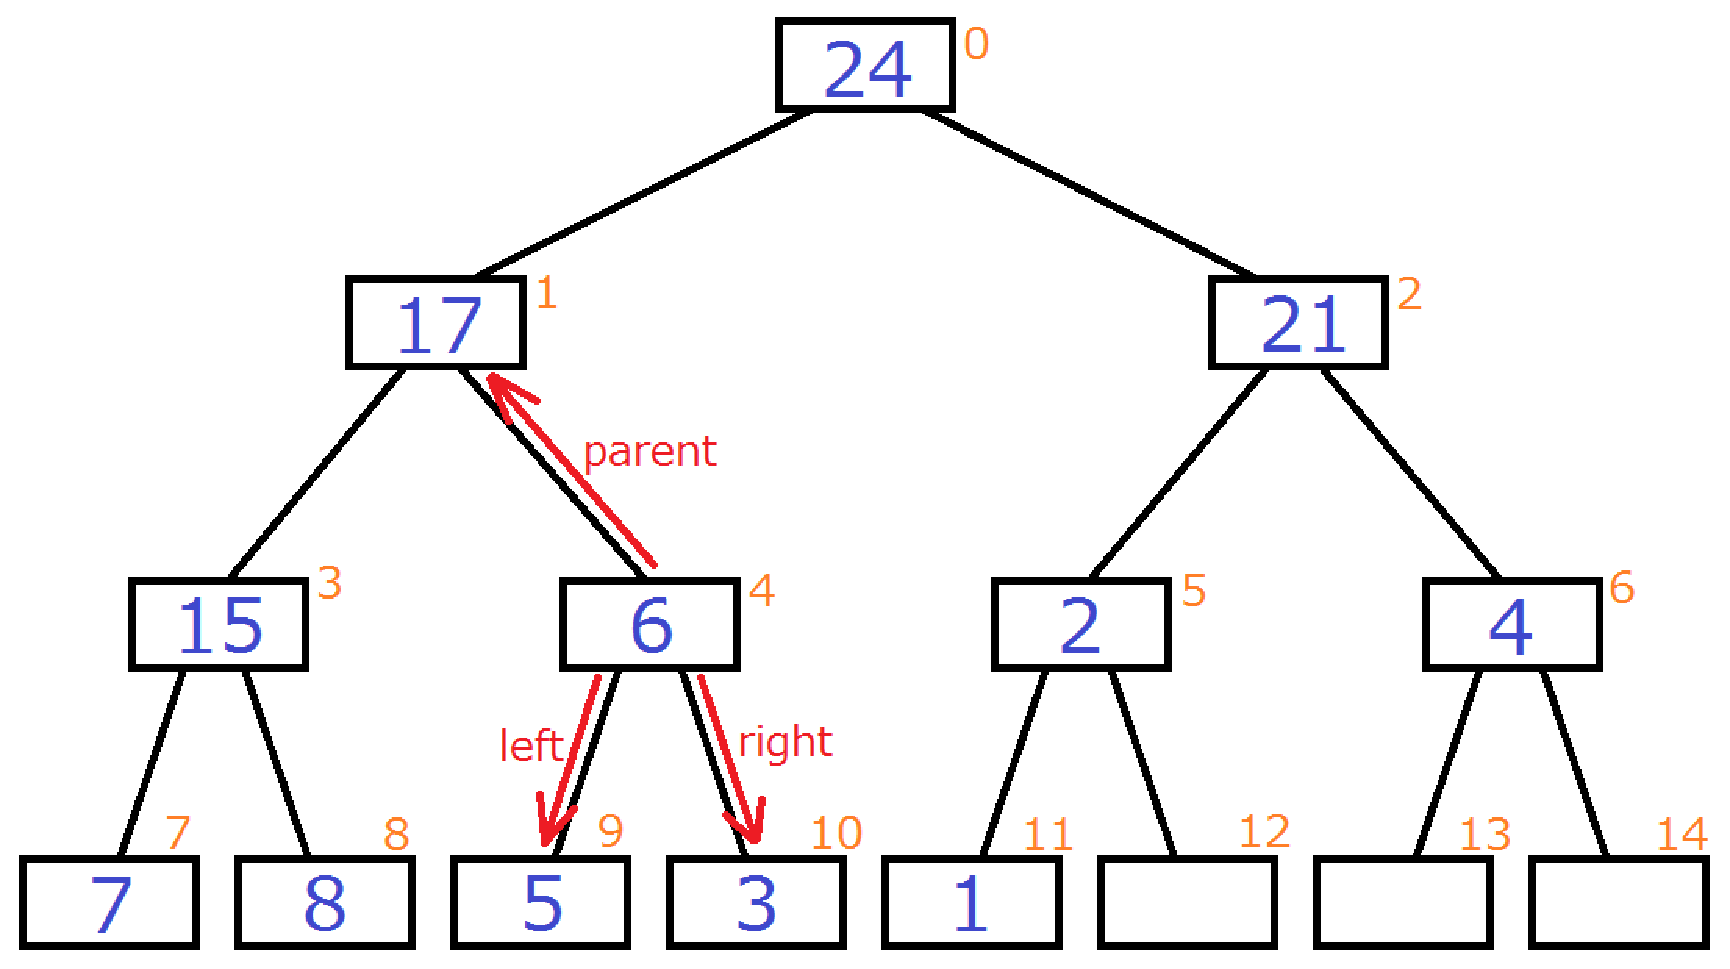
\includegraphics[width=8cm]{image/heap01.pdf}
    }
  \end{exampleblock}
}

\frame{
  \frametitle{push}
  \begin{block}{push}
    \center{
      $O(\log N)$で$C$の要素$x$を追加する
    }
  \end{block}
  \begin{exampleblock}{例}
    \center{
      \includegraphics<1>[width=8cm]{image/heap02.pdf}
      \includegraphics<2>[width=8cm]{image/heap03.pdf}
      \includegraphics<3>[width=8cm]{image/heap04.pdf}
    }
  \end{exampleblock}
}

\frame{
  \frametitle{replace}
  \begin{block}{replace}
    \center{
      $O(\log N)$で$C$の要素$x$ヒープの最大値をもつ要素を置き換える
    }
  \end{block}
  \begin{exampleblock}{例}
    \center{
      \includegraphics<1>[width=8cm]{image/heap05.pdf}
      \includegraphics<2>[width=8cm]{image/heap06.pdf}
      \includegraphics<3>[width=8cm]{image/heap07.pdf}
    }
  \end{exampleblock}
}

\frame{
  \frametitle{pop}
  \begin{block}{pop}
    \center{
      $O(\log N)$でヒープの最大値をもつ要素を削除する
    }
  \end{block}
  \begin{exampleblock}{例}
    \center{
      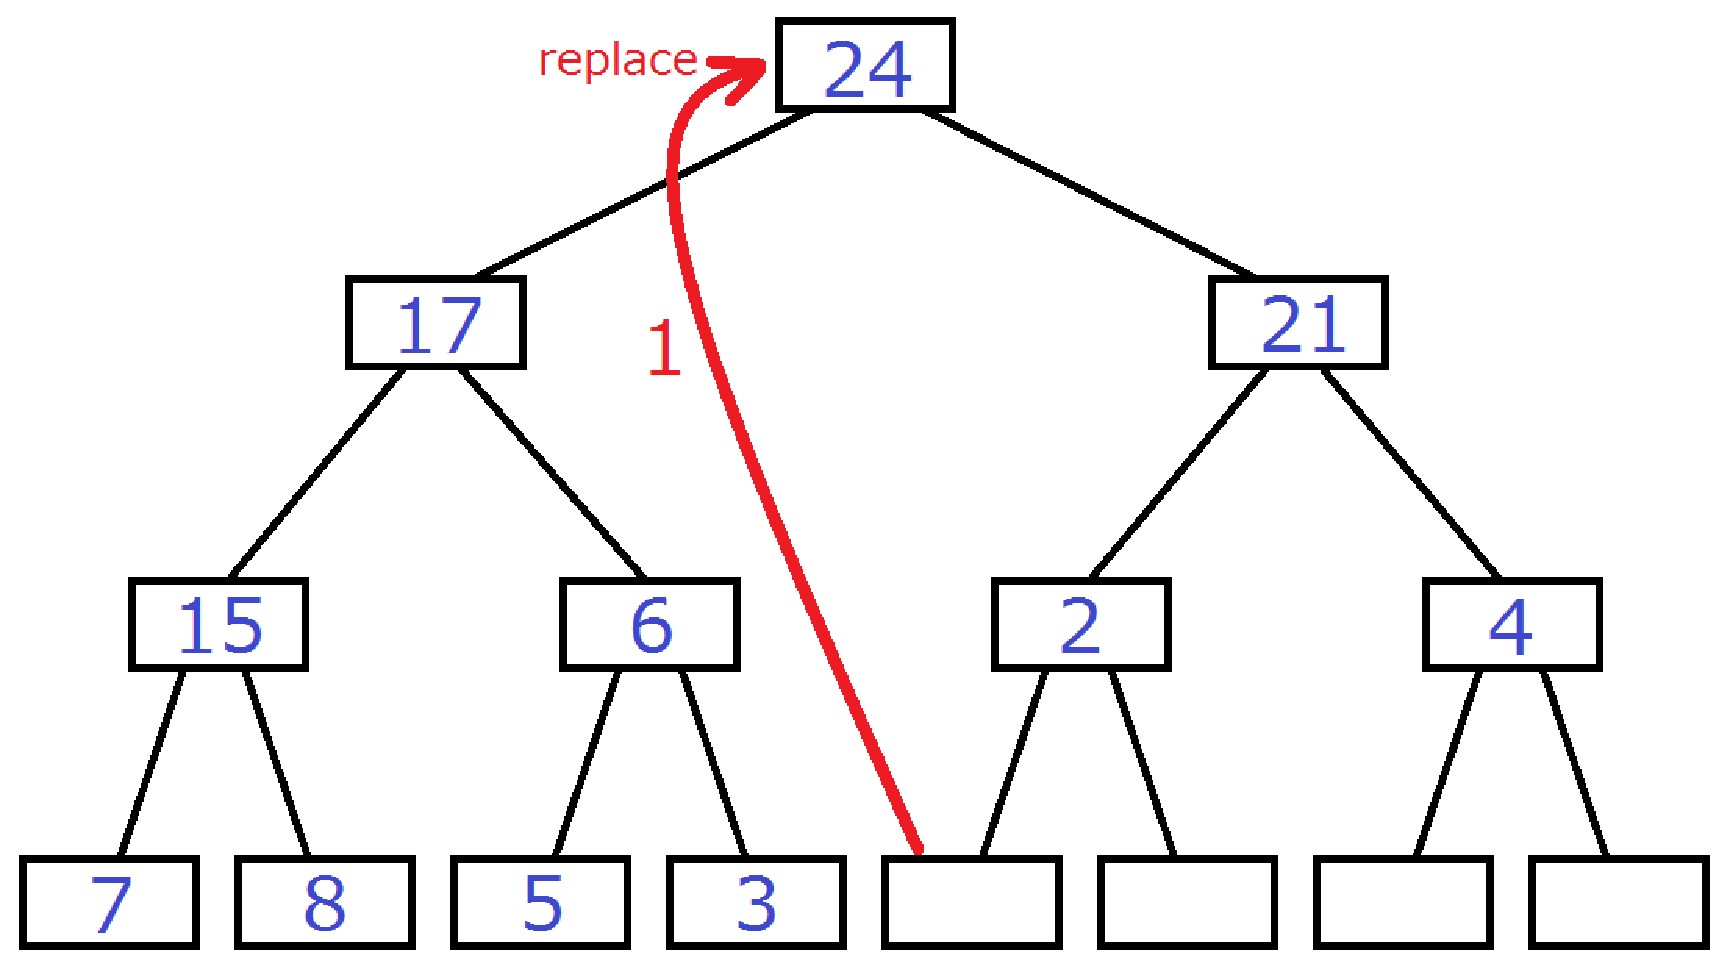
\includegraphics[width=8cm]{image/heap08.pdf}
    }
  \end{exampleblock}
}

\frame{
  \frametitle{delete}
  \begin{block}{delete}
    \center{
      $O(1)$で与えられたポインタの先の要素を消去する
    }
  \end{block}
  \begin{exampleblock}{例}
    \center{
      \includegraphics<1>[width=8cm]{image/heap09.pdf}
      \includegraphics<2>[width=8cm]{image/heap10.pdf}
      \includegraphics<3>[width=8cm]{image/heap11.pdf}
      \includegraphics<4>[width=8cm]{image/heap12.pdf}
      \includegraphics<5>[width=8cm]{image/heap13.pdf}
    }
  \end{exampleblock}
}

\frame{
  \frametitle{top}
  \begin{block}{top}
    \center{
      $O(1)$でヒープの最大値を求める\\ \\
    }
    ヒープの先頭の要素の値が最大値
  \end{block}
  \begin{alertblock}{ヒープは便利!!}
    ヒープを始めとする高速な優先度付きキューはあらゆる場面で活躍する
  \end{alertblock}
}
